\documentclass[11pt,a4paper]{article}

\usepackage[utf8]{inputenc}
\usepackage[T1]{fontenc}
\usepackage{lmodern}
\usepackage{microtype}
\usepackage{geometry}
\usepackage{setspace}
\usepackage{parskip}

\geometry{
    left=2.5cm,
    right=2.5cm,
    top=2.5cm,
    bottom=2.5cm
}
\onehalfspacing
\raggedbottom
\setlength{\emergencystretch}{3em}

\usepackage{graphicx}
\usepackage{float}
\usepackage{subcaption}
\graphicspath{{./}{./assets/}{./images/}}

\usepackage{tikz}
\usetikzlibrary{shapes.geometric, shapes.misc, arrows.meta, positioning, calc, fit, backgrounds}

\usepackage{listings}
\usepackage{xcolor}

\definecolor{codebg}{HTML}{F7F7F7}
\definecolor{codeframe}{HTML}{DDDDDD}
\definecolor{keyword}{HTML}{005FAF}
\definecolor{comment}{HTML}{6A737D}
\definecolor{string}{HTML}{D73A49}
\definecolor{accent}{HTML}{2E7D32}
\definecolor{warn}{HTML}{C62828}

\lstset{
    basicstyle=\ttfamily\footnotesize,
    keywordstyle=\color{keyword}\bfseries,
    commentstyle=\color{comment}\itshape,
    stringstyle=\color{string},
    numbers=left,
    numberstyle=\tiny\color{gray},
    backgroundcolor=\color{codebg},
    frame=single,
    rulecolor=\color{codeframe},
    breaklines=true,
    tabsize=4,
    showstringspaces=false,
    language=C++,
    aboveskip=1em,
    belowskip=1em
}

\usepackage{amsmath}
\usepackage{amssymb}

\usepackage{booktabs}
\usepackage{tabularx}
\usepackage{longtable}
\usepackage{etoolbox}
\usepackage{fancyvrb}

\usepackage{hyperref}
\hypersetup{
    colorlinks=true,
    linkcolor=black,
    urlcolor=keyword,
    citecolor=black,
    pdfauthor={Made Branenda Jordhy, Muhammad Nur Majiid, Jason Edward Salim, Athilla Zaidan Zidna Fann},
    pdftitle={Laporan Milestone 4 - Intermediate Code and Interpreter - IF2224}
}

% HEADER/FOOTER
\usepackage{fancyhdr}
\pagestyle{fancy}
\fancyhf{}
\setlength{\headheight}{36pt}
\fancyhead[L]{%
    \small\textnormal{School of Electrical Engineering and Informatics}\\[-1pt]
    \small\textnormal{Institut Teknologi Bandung}%
}
\fancyhead[R]{\IfFileExists{assets/LogoITB.png}{
\includegraphics[height=1cm]{assets/LogoITB.png}}{}}
\fancyfoot[L]{\small\textnormal{IF2224 Formal Language and Automata Theory}}
\fancyfoot[R]{\small\thepage}
\renewcommand{\headrulewidth}{0.4pt}
\renewcommand{\footrulewidth}{0.2pt}

% TITLE
\title{
    \vspace{-1.5cm}
    {\Large\textsc{IF2224 Formal Language and Automata Theory}}\\[0.35cm]
    {\LARGE\textbf{Arion Compiler - Milestone 4: Intermediate Code and Interpreter}}\\[0.3cm]
    \vspace{-0.3cm}
}
\author{}
\date{\today}

\begin{document}

\maketitle
\thispagestyle{empty}

\begin{figure}[H]
    \centering
    \IfFileExists{assets/foto_kelompok.png}{%
        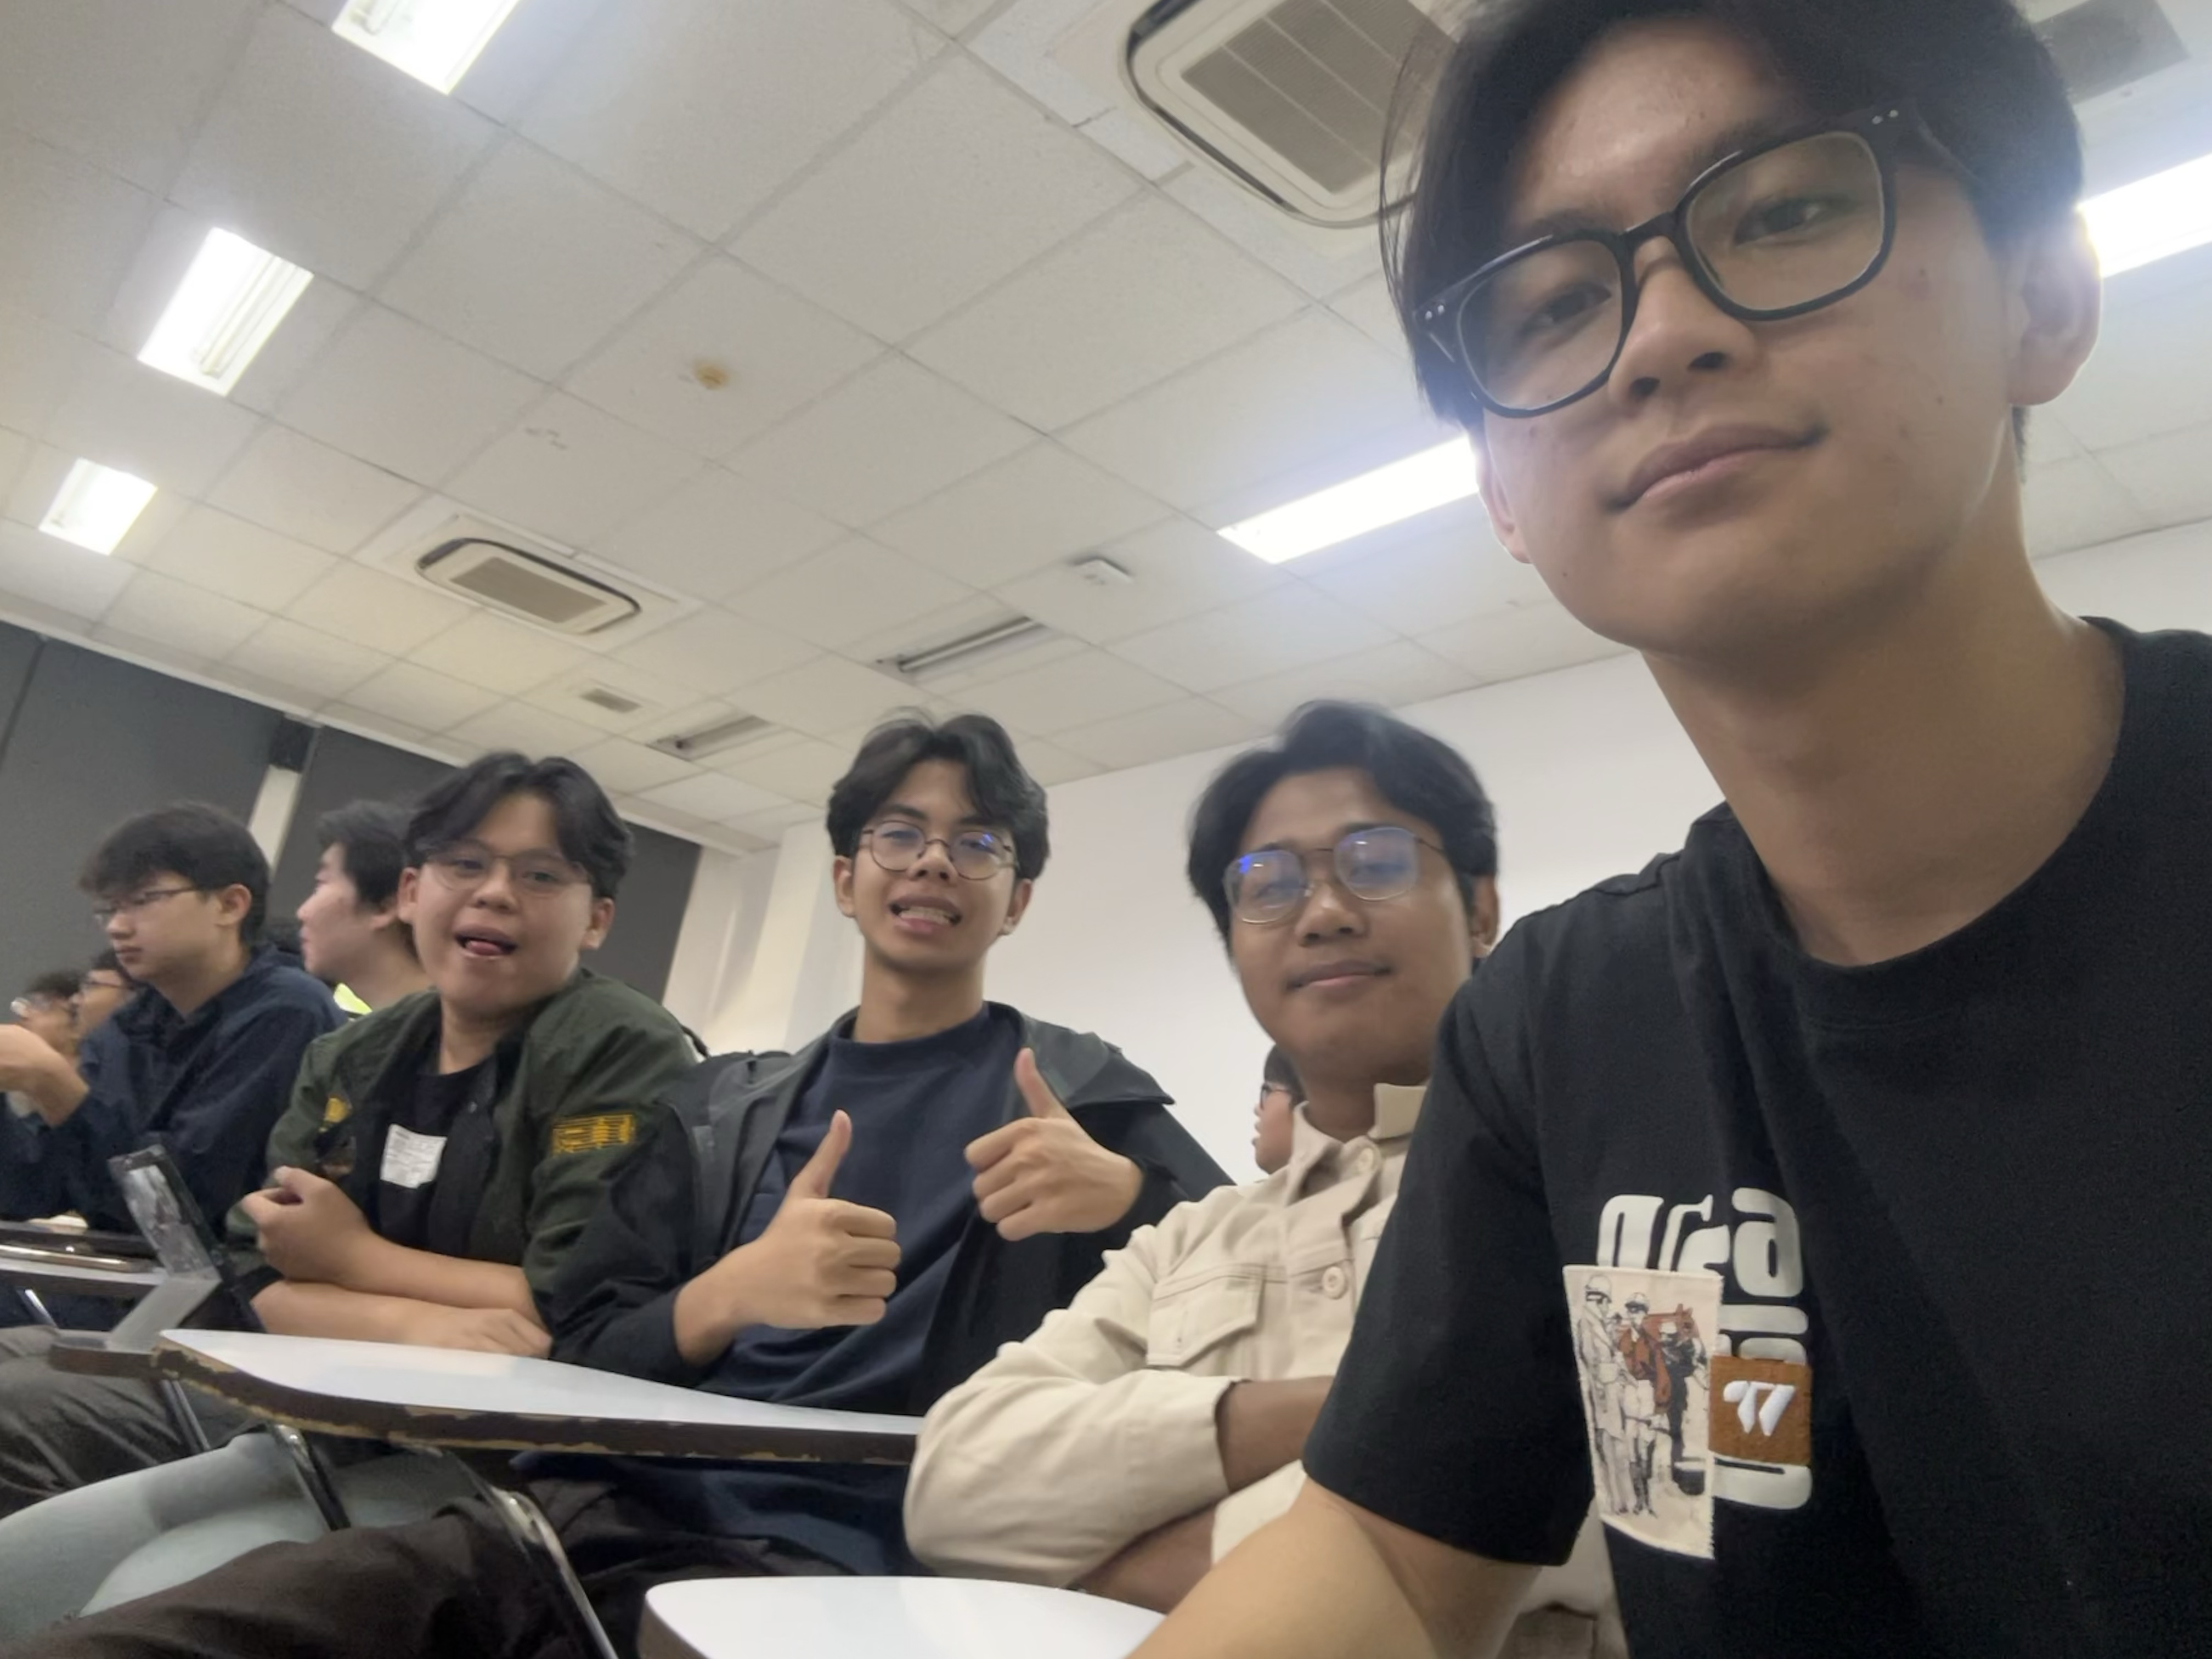
\includegraphics[width=0.6\textwidth]{assets/foto_kelompok.png}%
    }{%
        \vspace{4cm}
    }
\end{figure}

\vspace{1cm}
\begin{center}
    \textbf{Made Branenda Jordhy} - 13524026 \\[0.15cm]
    \textbf{Muhammad Nur Majiid} - 13524028 \\[0.15cm]
    \textbf{Jason Edward Salim} - 13524034 \\[0.15cm]
    \textbf{Athilla Zaidan Zidna Fann} - 13524068
\end{center}

\vspace{3cm}
\begin{center}
    {\large\textbf{School of Electrical Engineering and Informatics}}\\[0.1cm]
    {\large\textbf{Institut Teknologi Bandung}}\\[0.1cm]
    {\large\textbf{Semester II 2025/2026}}\\[0.1cm]
\end{center}

\newpage
\tableofcontents
\newpage

% =======================================================================
\section{Theoretical Background}

\subsection{Intermediate Code Generation}

\textit{Intermediate code generation} adalah tahap translasi dari
\textit{Decorated AST} menuju representasi instruksi yang lebih dekat dengan
mesin. Setelah Milestone~3, AST Arion sudah membawa informasi semantik seperti
tipe data, indeks symbol table, lexical level, dan alamat variabel. Informasi
tersebut menjadi dasar untuk mengubah ekspresi dan statement tingkat tinggi
menjadi instruksi linier~\cite{aho2006}.

Gambar~\ref{fig:dast} memperlihatkan contoh \textit{Decorated AST} untuk
statement \texttt{b := a + 10}. Setiap node tidak lagi sekadar merepresentasikan
struktur sintaksis, tetapi sudah dianotasi dengan tipe data hasil evaluasi dan
referensi ke entri symbol table (\texttt{tab\_index}). Anotasi inilah yang dibaca
oleh code generator untuk memutuskan instruksi yang tepat, misalnya memilih
\texttt{OPR ADD} untuk penjumlahan integer.

\begin{figure}[H]
\centering
\resizebox{0.82\textwidth}{!}{%
\begin{tikzpicture}[
    every node/.style={font=\small},
    astnode/.style={rectangle, draw, rounded corners=2pt, fill=codebg,
                    align=center, minimum height=0.9cm, inner sep=4pt},
    arr/.style={-{Stealth[length=2mm]}, thick, gray}
]
    \node[astnode] (assign) {Assign\\{\scriptsize\itshape\textcolor{accent}{type:void}}};
    \node[astnode, below left=1.2cm and 1.3cm of assign] (vb)
        {Var(b)\\{\scriptsize\itshape\textcolor{accent}{tab:35, type:int}}};
    \node[astnode, below right=1.2cm and 0.6cm of assign] (binop)
        {BinOp(+)\\{\scriptsize\itshape\textcolor{accent}{type:int}}};
    \node[astnode, below left=1.2cm and 0.1cm of binop] (va)
        {Var(a)\\{\scriptsize\itshape\textcolor{accent}{tab:34, type:int}}};
    \node[astnode, below right=1.2cm and 0.1cm of binop] (num)
        {Num(10)\\{\scriptsize\itshape\textcolor{accent}{type:int}}};
    \draw[arr] (assign) -- (vb);
    \draw[arr] (assign) -- (binop);
    \draw[arr] (binop) -- (va);
    \draw[arr] (binop) -- (num);
\end{tikzpicture}}
\caption{Decorated AST untuk \texttt{b := a + 10}; setiap node membawa anotasi
tipe dan indeks symbol table sebagai masukan code generator.}
\label{fig:dast}
\end{figure}

Pada Milestone~4 ini, bentuk instruksi yang digunakan mengikuti model
\textit{stack machine}. Setiap ekspresi dievaluasi dengan mendorong operand ke
stack, menjalankan operasi lewat instruksi \texttt{OPR}, lalu memakai nilai
hasilnya untuk assignment, percabangan, atau output. Pendekatan ini membuat
eksekusi tidak perlu lagi menelusuri pohon AST secara langsung.

\subsection{Three Address Code dan Stack Machine}

Secara umum, \textit{Three Address Code} memecah ekspresi kompleks menjadi
instruksi sederhana dengan jumlah operand terbatas. Pada implementasi Arion,
instruksi tidak menyimpan tiga alamat eksplisit seperti \texttt{t1 := a + b},
tetapi memakai bentuk P-Code sederhana:

\begin{center}
\begin{tabular}{c l c c}
\toprule
\textbf{Line} & \textbf{Instruksi} & \textbf{Level} & \textbf{Operand} \\
\midrule
0 & \texttt{INT} & 0 & 5 \\
1 & \texttt{LIT} & 0 & 5 \\
2 & \texttt{STO} & 0 & 3 \\
\bottomrule
\end{tabular}
\end{center}

Maknanya tetap sama: instruksi bekerja pada alamat memori dan stack. Instruksi
\texttt{LIT} mendorong literal ke stack, \texttt{LOD} membaca variabel,
\texttt{STO} menulis variabel, \texttt{CAL} membentuk frame pemanggilan,
\texttt{RET} membersihkan frame, \texttt{JMP}/\texttt{JPC} mengatur alur
kontrol, dan \texttt{OPR} menjalankan operasi aritmatika, relasional, atau
output.

Tabel~\ref{tab:icseq} menelusuri bagaimana ekspresi \texttt{y := (3 + 4) * x}
diratakan menjadi urutan instruksi sekaligus perubahan isi stack pada setiap
langkah~\cite{guidebook}. Operand terdalam dievaluasi lebih dahulu, lalu hasil
sementara ditumpuk hingga operasi terakhir menyisakan satu nilai yang disimpan
oleh \texttt{STO}.

\begin{table}[H]
\centering
\footnotesize
\begin{tabular}{c l l}
\toprule
\textbf{Langkah} & \textbf{Instruksi} & \textbf{Isi stack (atas $\rightarrow$ kanan)} \\
\midrule
1 & \texttt{LIT 3}   & $[\,3\,]$ \\
2 & \texttt{LIT 4}   & $[\,3,\,4\,]$ \\
3 & \texttt{OPR ADD} & $[\,7\,]$ \\
4 & \texttt{LOD x}   & $[\,7,\,\text{val\_x}\,]$ \\
5 & \texttt{OPR MUL} & $[\,7 \times \text{val\_x}\,]$ \\
6 & \texttt{STO y}   & $[\;]$ \quad (hasil disimpan ke \texttt{y}) \\
\bottomrule
\end{tabular}
\caption{Translasi ekspresi \texttt{y := (3 + 4) * x} menjadi urutan
intermediate code beserta evolusi isi stack.}
\label{tab:icseq}
\end{table}

Gambar~\ref{fig:stacktrace} menggambarkan evolusi stack tersebut secara visual
untuk ekspresi \texttt{a + 10} (dengan \texttt{a} bernilai 5): operand didorong,
dioperasikan oleh \texttt{OPR ADD}, lalu hasilnya disimpan.

\begin{figure}[H]
\centering
\begin{tikzpicture}[
    every node/.style={font=\footnotesize},
    cell/.style={draw, minimum width=1.1cm, minimum height=0.6cm, align=center},
    slbl/.style={font=\scriptsize\ttfamily},
    arr/.style={-{Stealth[length=2mm]}, thick}
]
    % stack 1: after LOD a -> [5]
    \node[cell, fill=codebg] (s1) at (0,0) {5};
    \node[slbl, below=0.15cm of s1] {LOD a};
    % stack 2: after LIT 10 -> [5,10]
    \node[cell, fill=codebg] (s2a) at (2.2,0) {5};
    \node[cell, fill=codebg] (s2b) at (2.2,0.6) {10};
    \node[slbl] at (2.2,-0.75) {LIT 10};
    % stack 3: after OPR ADD -> [15]
    \node[cell, fill=accent!15] (s3) at (4.4,0) {15};
    \node[slbl, below=0.15cm of s3] {OPR ADD};
    % stack 4: after STO b -> []
    \node[cell, draw, dashed] (s4) at (6.6,0) {\;};
    \node[slbl] at (6.6,-0.75) {STO b};

    \draw[arr] (s1.east) -- (1.65,0);
    \draw[arr] (3.05,0.3) -- (3.85,0.3);
    \draw[arr] (s3.east) -- (6.05,0);
\end{tikzpicture}
\caption{Aliran stack saat mengeksekusi \texttt{b := a + 10}: push operand,
\texttt{OPR ADD} menggantinya dengan hasil, lalu \texttt{STO} mengosongkan stack.}
\label{fig:stacktrace}
\end{figure}

\subsection{Interpreter}

Interpreter bertindak sebagai mesin virtual yang menjalankan daftar instruksi
secara berurutan. Mesin menyimpan tiga komponen utama:

\begin{itemize}
    \item \textbf{Instruction pointer} (\texttt{ip}) untuk menunjuk instruksi
          yang sedang dieksekusi.
    \item \textbf{Base pointer} (\texttt{bp}) untuk menunjuk awal stack frame
          aktif.
    \item \textbf{Stack} untuk menyimpan static link, dynamic link, return
          address, variabel lokal, parameter, operand sementara, dan hasil
          ekspresi.
\end{itemize}

Siklus eksekusinya mengikuti pola \textit{fetch-decode-execute}
(Gambar~\ref{fig:fde}). Interpreter mengambil instruksi pada \texttt{ip},
memeriksa opcode-nya, menjalankan handler yang sesuai, lalu melanjutkan ke
instruksi berikutnya kecuali terjadi lompatan atau return.

\begin{figure}[H]
\centering
\begin{tikzpicture}[
    every node/.style={font=\small},
    stage/.style={rectangle, draw, rounded corners=3pt, fill=codebg,
                  minimum width=2.6cm, minimum height=1.0cm, align=center},
    arr/.style={-{Stealth[length=2.5mm]}, thick}
]
    \node[stage] (fetch) {\textbf{Fetch}\\{\scriptsize ambil \texttt{code[ip]}}};
    \node[stage, right=1.6cm of fetch] (decode) {\textbf{Decode}\\{\scriptsize periksa opcode}};
    \node[stage, right=1.6cm of decode] (exec) {\textbf{Execute}\\{\scriptsize jalankan handler}};
    \draw[arr] (fetch) -- (decode);
    \draw[arr] (decode) -- (exec);
    \draw[arr] (exec) to[out=-90, in=-90, looseness=0.45]
        node[below, font=\scriptsize]{\texttt{ip++} atau lompat (\texttt{JMP}/\texttt{JPC}/\texttt{CAL}/\texttt{RET})} (fetch);
\end{tikzpicture}
\caption{Siklus \textit{fetch-decode-execute} pada interpreter Arion.}
\label{fig:fde}
\end{figure}

Secara konseptual, organisasi memori program mengikuti tata letak klasik pada
Gambar~\ref{fig:memlayout}: segmen \textit{text} menyimpan kode, segmen data
menyimpan variabel statis, sedangkan \textit{stack} (tempat frame fungsi Arion
hidup) tumbuh dari alamat tinggi ke rendah dan \textit{heap} tumbuh berlawanan
arah. Interpreter Arion berfokus pada segmen \textit{stack}.

\begin{figure}[H]
\centering
\begin{tikzpicture}[
    seg/.style={rectangle, draw, minimum width=4.2cm, minimum height=0.85cm,
                align=center, font=\small}
]
    \node[seg, fill=orange!18] (stack) at (0,4.0) {Stack {\scriptsize(tumbuh ke bawah)}};
    \node[font=\scriptsize] at (0,3.25) {$\downarrow \quad\cdots\quad \uparrow$};
    \node[seg, fill=green!12] (heap) at (0,2.5) {Heap {\scriptsize(tumbuh ke atas)}};
    \node[seg, fill=blue!8]  (bss)  at (0,1.6) {Uninitialized Data (BSS)};
    \node[seg, fill=blue!14] (data) at (0,0.75) {Initialized Data};
    \node[seg, fill=red!12]  (text) at (0,-0.1) {Text {\scriptsize(kode program)}};
    \node[font=\scriptsize, right=0.35cm of stack] {High address};
    \node[font=\scriptsize, right=0.35cm of text] {Low address};
\end{tikzpicture}
\caption{Tata letak memori program; interpreter Arion mengelola segmen
\textit{stack} untuk frame, operand, dan hasil sementara.}
\label{fig:memlayout}
\end{figure}

\subsection{Runtime Safety}

Walaupun Arion sudah melakukan pengecekan semantik secara statis, interpreter
tetap perlu menjaga keamanan eksekusi. Implementasi saat ini menambahkan
pengecekan \textit{stack overflow}, \textit{stack underflow}, akses stack
\textit{out-of-bounds}, target jump invalid, pembagian dengan nol, modulo dengan
nol, serta opcode/OPR yang tidak dikenal. Dengan demikian, kesalahan runtime
tidak langsung menyebabkan program C++ crash, tetapi dilaporkan melalui
\texttt{RuntimeError}.

% =======================================================================
\section{Design and Implementation}

\subsection{Overview Pipeline}

Pipeline kompilasi yang menjadi dasar Milestone~4 adalah kelanjutan dari tiga
milestone sebelumnya. Lexer menghasilkan token stream, parser membangun parse
tree, AST builder mereduksi parse tree menjadi AST, semantic analyzer
mendekorasi AST dan mengisi symbol table, lalu code generator membuat
intermediate code yang dapat dijalankan interpreter.

\begin{figure}[H]
\centering
\resizebox{\textwidth}{!}{%
\begin{tikzpicture}[
    every node/.style={font=\small},
    src/.style={rectangle, draw, fill=codebg, rounded corners=2pt,
                minimum width=2.5cm, minimum height=0.85cm, align=center},
    proc/.style={rectangle, draw, fill=yellow!12, rounded corners=2pt,
                 minimum width=2.5cm, minimum height=0.85cm, align=center},
    back/.style={rectangle, draw, fill=accent!15, rounded corners=2pt,
                 minimum width=2.5cm, minimum height=0.85cm, align=center},
    arr/.style={-{Stealth[length=2.5mm]}, thick}
]
    \node[src]  (src) at (0,0) {Source};
    \node[proc, right=0.55cm of src] (lex) {Lexer};
    \node[proc, right=0.55cm of lex] (par) {Parser};
    \node[proc, right=0.55cm of par] (ast) {AST Builder};
    \node[proc, right=0.55cm of ast] (sem) {Semantic\\Analyzer};
    \node[back, right=0.55cm of sem] (cg) {Code\\Generator};
    \node[back, right=0.55cm of cg] (vm) {Interpreter};
    \node[src, right=0.55cm of vm] (out) {Output};

    \draw[arr] (src) -- (lex);
    \draw[arr] (lex) -- (par);
    \draw[arr] (par) -- (ast);
    \draw[arr] (ast) -- (sem);
    \draw[arr] (sem) -- (cg);
    \draw[arr] (cg) -- (vm);
    \draw[arr] (vm) -- (out);
\end{tikzpicture}}
\caption{Pipeline lengkap Arion dari source code hingga output eksekusi.}
\label{fig:pipeline}
\end{figure}

\subsection{Instruction Representation}

Instruksi intermediate code didefinisikan pada \texttt{src/header/instruction.hpp}
dengan empat field utama: nomor baris, opcode, level, dan operand.

\begin{lstlisting}
struct Instruction {
    int line;
    OpCode op;
    int level;
    int operand;
};
\end{lstlisting}

Opcode yang tersedia dirangkum pada Tabel~\ref{tab:opcode}. Instruksi ini
sesuai dengan konvensi pada spesifikasi Milestone~4, dengan tambahan struktur
data C++ agar mudah dicetak dan dieksekusi.

\begin{table}[H]
\centering
\begin{tabularx}{\textwidth}{l X}
\toprule
\textbf{Opcode} & \textbf{Fungsi} \\
\midrule
\texttt{INT} & Mengalokasikan ruang variabel lokal pada stack frame aktif. Frame header dibuat saat inisialisasi global atau saat \texttt{CAL}. \\
\texttt{LIT} & Mendorong nilai literal integer/boolean/char ke stack. \\
\texttt{LOD} & Membaca nilai variabel dari stack frame tertentu. \\
\texttt{STO} & Mengambil nilai dari puncak stack dan menyimpannya ke alamat variabel. \\
\texttt{CAL} & Melakukan pemanggilan prosedur/fungsi. \\
\texttt{JMP} & Melompat tanpa syarat ke baris instruksi tertentu. \\
\texttt{JPC} & Melompat jika kondisi pada puncak stack bernilai false/0. \\
\texttt{OPR} & Menjalankan operasi aritmatika, relasional, atau output. \\
\texttt{RET} & Keluar dari stack frame aktif dan kembali ke caller. \\
\bottomrule
\end{tabularx}
\caption{Opcode intermediate code yang tersedia.}
\label{tab:opcode}
\end{table}

\subsection{OPR Code}

Instruksi \texttt{OPR} memakai operand sebagai kode operasi. Operasi yang
diimplementasikan adalah \texttt{NEG}, \texttt{ADD}, \texttt{SUB},
\texttt{MUL}, \texttt{DIV}, \texttt{MOD}, operator relasional
\texttt{EQL}/\texttt{NEQ}/\texttt{LSS}/\texttt{GEQ}/\texttt{GTR}/\texttt{LEQ},
serta \texttt{WRT} dan \texttt{WRTLN}. Nilai boolean direpresentasikan sebagai
integer \texttt{0} dan \texttt{1}, sehingga operasi \texttt{and} dipetakan ke
perkalian dan \texttt{or} dipetakan ke penjumlahan pada code generator.
Tabel~\ref{tab:opr} merangkum seluruh kode operasi \texttt{OPR}.

\begin{table}[H]
\centering
\footnotesize
\begin{tabularx}{\textwidth}{c l X c l X}
\toprule
\textbf{No} & \textbf{Op} & \textbf{Fungsi} & \textbf{No} & \textbf{Op} & \textbf{Fungsi} \\
\midrule
1 & \texttt{NEG} & negasi unary      & 8  & \texttt{NEQ}   & tidak sama dengan \\
2 & \texttt{ADD} & penjumlahan       & 9  & \texttt{LSS}   & lebih kecil \\
3 & \texttt{SUB} & pengurangan       & 10 & \texttt{GEQ}   & lebih besar sama dengan \\
4 & \texttt{MUL} & perkalian         & 11 & \texttt{GTR}   & lebih besar \\
5 & \texttt{DIV} & pembagian integer & 12 & \texttt{LEQ}   & lebih kecil sama dengan \\
6 & \texttt{MOD} & modulo            & 13 & \texttt{WRT}   & cetak nilai \\
7 & \texttt{EQL} & sama dengan       & 14 & \texttt{WRTLN} & cetak nilai + newline \\
\bottomrule
\end{tabularx}
\caption{Kode operasi pada instruksi \texttt{OPR} (operand = nomor operasi).}
\label{tab:opr}
\end{table}

\subsection{Code Generator}

Komponen \texttt{CodeGenerator} berada pada \texttt{src/header/codegen.hpp} dan
\texttt{src/lib/codegen.cpp}. Generator menerima \texttt{ASTNode*} dan
\texttt{SymbolTable} hasil semantic analyzer. Sebelum menghasilkan instruksi,
generator memanggil \texttt{resolveAddresses()} untuk mengisi alamat variabel
pada \texttt{tab[idx].adr} berdasarkan urutan deklarasi pada setiap
\texttt{btab}.

Strategi translasi dilakukan secara rekursif sesuai jenis node AST:

\begin{itemize}
    \item \texttt{genProgram()} menghasilkan instruksi utama dan, bila ada
          subprogram, membuat \texttt{JMP} awal untuk melewati kode prosedur
          atau fungsi.
    \item \texttt{genAssign()} menghasilkan instruksi ekspresi kanan lalu
          \texttt{STO} ke alamat variabel target.
    \item \texttt{genIf()} memakai \texttt{JPC} yang di-\textit{patch} setelah
          cabang \texttt{then}/\texttt{else} selesai digenerate.
    \item \texttt{genWhile()}, \texttt{genFor()}, dan \texttt{genRepeat()}
          membangun control flow dengan kombinasi label implisit berupa nomor
          baris, \texttt{JMP}, dan \texttt{JPC}.
    \item \texttt{genCall()} menangani \texttt{write}/\texttt{writeln} sebagai
          \texttt{OPR WRT/WRTLN}, dan subprogram pengguna sebagai
          \texttt{CAL}.
\end{itemize}

Tantangan utama pada \textit{control flow} adalah meratakan blok bersarang
menjadi instruksi linier menggunakan \textit{label} (nomor baris) dan
\textit{jump}. Gambar~\ref{fig:ctrlflow} memperlihatkan pola translasi
\texttt{if-else} dan \texttt{while}. Pada \texttt{if-else}, \texttt{JPC}
melompat ke cabang \texttt{else} bila kondisi bernilai \textit{false}, dan
\texttt{JMP} melewati cabang \texttt{else} setelah \texttt{then} selesai. Pada
\texttt{while}, kondisi dievaluasi ulang setiap iterasi dan \texttt{JMP}
kembali ke label awal.

\begin{figure}[H]
\centering
\begin{subfigure}[t]{0.48\textwidth}
\centering
\resizebox{\textwidth}{!}{%
\begin{tikzpicture}[
    every node/.style={font=\small},
    blk/.style={rectangle, draw, rounded corners=2pt, fill=codebg,
                minimum width=3.2cm, minimum height=0.7cm, align=center},
    arr/.style={-{Stealth[length=2mm]}, thick},
    jmp/.style={-{Stealth[length=2mm]}, thick, warn, dashed}
]
    \node[blk] (cond) {evaluasi kondisi};
    \node[blk, below=0.45cm of cond] (jpc) {\texttt{JPC L\_else}};
    \node[blk, below=0.45cm of jpc] (then) {kode \texttt{then}};
    \node[blk, below=0.45cm of then] (jmp) {\texttt{JMP L\_end}};
    \node[blk, below=0.45cm of jmp, fill=yellow!12] (els) {kode \texttt{else}};
    \node[blk, below=0.45cm of els, fill=accent!12] (end) {\texttt{L\_end}};
    \draw[arr] (cond) -- (jpc);
    \draw[arr] (jpc) -- (then);
    \draw[arr] (then) -- (jmp);
    \draw[jmp] (jpc.east) to[out=0,in=0,looseness=1.4] (els.east);
    \draw[jmp] (jmp.west) to[out=180,in=180,looseness=1.4] (end.west);
\end{tikzpicture}}
\caption{\texttt{if-else}}
\end{subfigure}
\hfill
\begin{subfigure}[t]{0.48\textwidth}
\centering
\resizebox{\textwidth}{!}{%
\begin{tikzpicture}[
    every node/.style={font=\small},
    blk/.style={rectangle, draw, rounded corners=2pt, fill=codebg,
                minimum width=3.2cm, minimum height=0.7cm, align=center},
    arr/.style={-{Stealth[length=2mm]}, thick},
    jmp/.style={-{Stealth[length=2mm]}, thick, warn, dashed}
]
    \node[blk, fill=accent!12] (start) {\texttt{L\_start}};
    \node[blk, below=0.45cm of start] (cond) {evaluasi kondisi};
    \node[blk, below=0.45cm of cond] (jpc) {\texttt{JPC L\_end}};
    \node[blk, below=0.45cm of jpc] (body) {kode \texttt{body}};
    \node[blk, below=0.45cm of body] (jmp) {\texttt{JMP L\_start}};
    \node[blk, below=0.45cm of jmp, fill=accent!12] (end) {\texttt{L\_end}};
    \draw[arr] (start) -- (cond);
    \draw[arr] (cond) -- (jpc);
    \draw[arr] (jpc) -- (body);
    \draw[arr] (body) -- (jmp);
    \draw[jmp] (jmp.east) to[out=0,in=0,looseness=1.6] (start.east);
    \draw[jmp] (jpc.west) to[out=180,in=180,looseness=1.4] (end.west);
\end{tikzpicture}}
\caption{\texttt{while}}
\end{subfigure}
\caption{Pola translasi \textit{control flow}; panah putus-putus merah adalah
lompatan (\texttt{JPC}/\texttt{JMP}).}
\label{fig:ctrlflow}
\end{figure}

Generator juga sudah memisahkan alamat parameter dan variabel lokal. Parameter
disimpan pada alamat negatif relatif terhadap base pointer, sedangkan variabel
lokal dimulai dari offset \texttt{FRAME\_HEADER\_SIZE}. Pada fungsi, assignment
ke nama fungsi dibaca kembali sebagai nilai return dan diikuti instruksi
\texttt{RET 1 psze}; pada prosedur, instruksi akhirnya adalah
\texttt{RET 0 psze}. Operand \texttt{psze} dipakai interpreter untuk
membersihkan argumen setelah subprogram selesai.

\begin{figure}[H]
\centering
\begin{tikzpicture}[
    every node/.style={font=\small},
    proc/.style={rectangle, draw, fill=codebg, rounded corners=2pt,
                 minimum width=3.3cm, minimum height=0.75cm},
    dec/.style={diamond, draw, fill=yellow!12, aspect=2.5,
                minimum width=2.8cm, minimum height=0.9cm},
    arr/.style={-{Stealth[length=2.5mm]}, thick},
    lbl/.style={font=\scriptsize, fill=white, inner sep=1pt}
]
    \node[proc] (start) {genExpr(left)};
    \node[proc, below=0.8cm of start] (right) {genExpr(right)};
    \node[dec, below=0.9cm of right] (op) {operator?};
    \node[proc, below left=1.0cm and 0.5cm of op] (arith) {emit OPR arithmetic};
    \node[proc, below right=1.0cm and 0.5cm of op] (rel) {emit OPR relational};

    \draw[arr] (start) -- (right);
    \draw[arr] (right) -- (op);
    \draw[arr] (op) -- node[lbl, left] {+ - * div mod} (arith);
    \draw[arr] (op) -- node[lbl, right] {== <> < <= > >=} (rel);
\end{tikzpicture}
\caption{Skema translasi ekspresi biner pada code generator.}
\label{fig:binop}
\end{figure}

\subsection{Interpreter}

Komponen \texttt{Interpreter} diimplementasikan sebagai modul header dan
library terpisah. Interpreter menyimpan daftar instruksi, stack eksekusi,
serta pointer \texttt{ip} dan \texttt{bp}. Setiap opcode memiliki handler
terpisah untuk operasi literal, load, store, call, jump, conditional jump,
operasi \texttt{OPR}, dan return.

Stack frame menggunakan tiga slot awal. Pada awal eksekusi, interpreter
mendorong frame header global berisi tiga nol. Pada pemanggilan subprogram,
\texttt{CAL} mendorong static link, dynamic link, dan return address, lalu
\texttt{INT} menambahkan ruang lokal.

Struktur frame ditunjukkan pada Gambar~\ref{fig:frame}. Tiga slot pertama
(\textit{offset} 0--2) berisi static link, dynamic link, dan return address.
Variabel lokal menempati \textit{offset} positif mulai dari
\texttt{FRAME\_HEADER\_SIZE} (3), sedangkan parameter berada pada \textit{offset}
negatif relatif terhadap \texttt{BP} karena di-\textit{push} oleh pemanggil
sebelum \texttt{CAL}.

\begin{figure}[H]
\centering
\begin{tikzpicture}[
    every node/.style={font=\small},
    slot/.style={rectangle, draw, minimum width=6.2cm, minimum height=0.72cm,
                 align=center},
    ptr/.style={-{Stealth[length=2.5mm]}, thick}
]
    \node[slot, fill=orange!14] (sp)   at (0,4.32) {operand kerja / hasil ekspresi \quad $\cdots$};
    \node[slot, fill=codebg]    (loc)  at (0,3.60) {\textit{offset} 3, 4, $\dots$ : variabel lokal};
    \node[slot, fill=blue!8]    (ra)   at (0,2.88) {\textit{offset} 2 : return address};
    \node[slot, fill=blue!8]    (dl)   at (0,2.16) {\textit{offset} 1 : dynamic link (BP pemanggil)};
    \node[slot, fill=blue!8]    (sl)   at (0,1.44) {\textit{offset} 0 : static link};
    \node[slot, fill=green!12]  (par)  at (0,0.62) {\textit{offset} $-1, -2, \dots$ : parameter};
    \draw[ptr] ($(sl.east)+(1.4,0)$) node[right, font=\scriptsize]{\texttt{BP}} -- (sl.east);
    \draw[ptr] ($(sp.east)+(1.4,0)$) node[right, font=\scriptsize]{\texttt{SP}} -- (sp.east);
\end{tikzpicture}
\caption{Struktur stack frame Arion: header (SL, DL, RA), variabel lokal pada
\textit{offset} positif, dan parameter pada \textit{offset} negatif.}
\label{fig:frame}
\end{figure}

Alamat variabel dihitung lewat \texttt{resolveAddress(level, address)}. Nilai
\texttt{level} menyatakan berapa banyak static link yang perlu ditelusuri dari
frame aktif untuk mencapai frame deklarasi variabel. Mekanisme ini penting untuk
\textit{nested scope}: Gambar~\ref{fig:staticlink} memperlihatkan rantai static
link ketika prosedur \texttt{Inner} (level~2) mengakses variabel milik
\texttt{Outer} (level~1) atau variabel global (level~0).

\begin{figure}[H]
\centering
\begin{tikzpicture}[
    every node/.style={font=\small},
    frame/.style={rectangle, draw, rounded corners=2pt, minimum width=3.6cm,
                  minimum height=1.0cm, align=center},
    sl/.style={-{Stealth[length=2.5mm]}, thick, keyword}
]
    \node[frame, fill=red!8]   (main)  at (0,0)   {Frame \texttt{main} \\ {\scriptsize level 0 (global)}};
    \node[frame, fill=blue!8]  (outer) at (0,1.7) {Frame \texttt{Outer} \\ {\scriptsize level 1}};
    \node[frame, fill=green!12](inner) at (0,3.4) {Frame \texttt{Inner} \\ {\scriptsize level 2}};
    \draw[sl] (inner.west) to[out=180,in=180,looseness=1.6]
        node[left, font=\scriptsize]{SL} (outer.west);
    \draw[sl] (outer.east) to[out=0,in=0,looseness=1.6]
        node[right, font=\scriptsize]{SL} (main.east);
\end{tikzpicture}
\caption{Rantai static link pada \textit{nested scope}. Akses \texttt{LOD}
dengan \texttt{level} = (level pemakai $-$ level deklarasi) menelusuri rantai ini.}
\label{fig:staticlink}
\end{figure}

\subsection{Error Handling}

Pada code generator, error dilaporkan dengan \texttt{CodeGenError}. Contoh
kasus yang ditangani adalah target assignment yang belum ter-resolve, literal
real yang belum didukung oleh stack machine, \texttt{readln} yang belum
diimplementasikan, dan operator yang belum dipetakan ke \texttt{OPR}.

Pada interpreter, error runtime dilaporkan dengan \texttt{RuntimeError}. Handler
mengecek batas stack, stack kosong sebelum operasi \texttt{pop}, target jump di
luar range instruksi, frame pointer invalid, pembagian dengan nol, modulo dengan
nol, dan kode \texttt{OPR} yang tidak dikenal. Tabel~\ref{tab:runtime}
merangkum skema validasi runtime tersebut.

\begin{table}[H]
\centering
\footnotesize
\begin{tabularx}{\textwidth}{l X X}
\toprule
\textbf{Kondisi} & \textbf{Mekanisme deteksi} & \textbf{Tindakan} \\
\midrule
Stack Overflow  & cek \texttt{SP} terhadap \texttt{MAX\_STACK\_SIZE} & \texttt{RuntimeError}: stack overflow \\
Stack Underflow & cek stack kosong sebelum \texttt{pop} & \texttt{RuntimeError}: stack underflow \\
Invalid Jump    & validasi target \texttt{JMP}/\texttt{JPC}/\texttt{CAL} terhadap rentang instruksi & \texttt{RuntimeError}: invalid jump target \\
OOB Access      & cek alamat pada \texttt{LOD}/\texttt{STO} terhadap batas stack & \texttt{RuntimeError}: out-of-bounds stack access \\
Division/Modulo by Zero & cek pembagi bernilai nol pada \texttt{DIV}/\texttt{MOD} & \texttt{RuntimeError}: division/modulo by zero \\
Type Mismatch   & atribut tipe pada Decorated AST (statis, di M3) & hentikan kompilasi, pesan error tipe \\
\bottomrule
\end{tabularx}
\caption{Skema validasi runtime pada interpreter Arion.}
\label{tab:runtime}
\end{table}

Sebagai ilustrasi, Gambar~\ref{fig:overflow} menunjukkan kondisi
\textit{stack overflow} akibat rekursi tanpa \textit{base case}: setiap
pemanggilan menambah frame baru hingga \texttt{SP} melampaui
\texttt{MAX\_STACK\_SIZE}, dan interpreter melempar \texttt{RuntimeError}
sebelum memori benar-benar rusak.

\begin{figure}[H]
\centering
\begin{tikzpicture}[
    every node/.style={font=\footnotesize},
    fr/.style={rectangle, draw, minimum width=3.4cm, minimum height=0.55cm,
               align=center, fill=codebg},
    arr/.style={-{Stealth[length=2.5mm]}, thick, warn}
]
    \node[fr] (f1) at (0,0)    {frame \texttt{f} \#1};
    \node[fr] (f2) at (0,0.6)  {frame \texttt{f} \#2};
    \node[fr] (f3) at (0,1.2)  {frame \texttt{f} \#3};
    \node[fr] (f4) at (0,1.8)  {frame \texttt{f} \#4};
    \node[font=\footnotesize] (dots) at (0,2.45) {$\vdots$ \;\; (terus bertambah)};
    \draw[dashed, warn, thick] (-2.0,2.95) -- (2.0,2.95)
        node[right, font=\scriptsize]{\texttt{MAX\_STACK\_SIZE}};
    \node[fr, fill=warn!18] (fx) at (0,3.35) {frame \texttt{f} \#N};
    \draw[arr] (2.3,0) -- node[right, font=\scriptsize]{SP naik} (2.3,3.35);
    \node[warn, font=\scriptsize\bfseries, right=0.2cm of fx] {Stack Overflow!};
\end{tikzpicture}
\caption{Ilustrasi \textit{stack overflow} pada rekursi tak hingga; interpreter
mendeteksi \texttt{SP} melewati batas dan menghentikan eksekusi dengan aman.}
\label{fig:overflow}
\end{figure}

\subsection{Status Integrasi}

Berdasarkan struktur repository saat laporan ini dibuat, komponen Milestone~4
sudah terintegrasi ke pipeline utama. \texttt{Makefile} telah memasukkan
\path{src/lib/codegen.cpp} dan \path{src/lib/interpreter.cpp} ke daftar
\texttt{SRC}. Sementara itu, \path{src/main.cpp} sudah menghubungkan
\texttt{codegen.hpp} dan \texttt{interpreter.hpp}. Setelah lexer, parser, AST
builder, dan semantic analyzer selesai, program menghasilkan intermediate code
melalui \texttt{CodeGenerator}, mencetaknya, lalu menjalankannya melalui
\texttt{Interpreter} pada bagian \texttt{--- Output Program ---}.

Dengan demikian, executable utama tidak lagi berhenti pada \textit{Decorated
AST}. Output terminal sudah berisi seluruh tahapan: daftar token, parse tree,
decorated AST, symbol table, intermediate code, dan output aktual program Arion.

Keterbatasan implementasi yang terlihat dari kode adalah sebagai berikut.

\begin{itemize}
    \item Eksekusi stack machine masih berbasis \texttt{int}; literal
          \texttt{real} belum didukung.
    \item \texttt{writeln} untuk string literal di-skip oleh generator, sehingga
          output string belum tersedia pada stack machine.
    \item Assignment baru mendukung variabel sederhana; akses array dan field
          record belum digenerate.
    \item \texttt{readln} belum didukung pada code generation.
    \item \texttt{case} belum memiliki cabang generator khusus.
\end{itemize}

% =======================================================================
\section{Testing}

Pengujian (\textit{testing}) Milestone~4 disimpan pada direktori
\texttt{test/milestone-4/}. Setiap testcase memiliki berkas input dan output
dengan format \texttt{input-\{n\}.txt} dan
\texttt{output/output-\{n\}.txt}. Output pada folder tersebut berbentuk
intermediate code teks, sehingga dapat langsung dimasukkan ke laporan dengan
\texttt{lstinputlisting}.

\subsection{Lokasi File Pengujian}

\begin{itemize}
    \item file input: \path{test/milestone-4/input-1.txt} s.d. \path{test/milestone-4/input-8.txt}
    \item file output: \path{test/milestone-4/output/output-1.txt} s.d. \path{test/milestone-4/output/output-8.txt}
\end{itemize}

\subsection{Ringkasan Kasus Uji}

\begin{table}[H]
\centering
\footnotesize
\begin{tabularx}{\textwidth}{c l X c}
\toprule
\textbf{No} & \textbf{Fokus} & \textbf{Deskripsi singkat} & \textbf{Output} \\
\midrule
1 & Assignment dasar & Assignment integer, operasi penjumlahan, dan \texttt{writeln}. & \texttt{15} \\
2 & \texttt{if-else} dan \texttt{while} & Percabangan dengan \texttt{JPC}/\texttt{JMP}, operasi relasional, dan loop decrement. & \texttt{0} \\
3 & \texttt{for} dan \texttt{repeat-until} & Translasi \texttt{for-to}, akumulasi nilai, dan loop \texttt{repeat} sampai kondisi terpenuhi. & \texttt{15, 0} \\
4 & Function call & Contoh instruksi \texttt{JMP} awal, entry fungsi, \texttt{CAL}, dan \texttt{RET}. & \texttt{25} \\
5 & Nested scope & Contoh static link dan akses variabel pada lexical level berbeda. & --- \\
6 & Procedure call dengan parameter & Pemanggilan prosedur \texttt{add(a,b)}, parameter alamat negatif, dan pembersihan argumen lewat \texttt{RET 0 2}. & \texttt{30, 30} \\
7 & Nested procedure dan loop & Prosedur dengan parameter, \texttt{if-else}, \texttt{while}, dan dua kali pemanggilan dari blok utama. & \texttt{5, 0, 26, 0} \\
8 & Aritmatika lengkap & Operasi \texttt{+}, \texttt{-}, \texttt{*}, \texttt{div}, relasional \texttt{<}, dan beberapa output. & \texttt{15, 5, 50, 2, 5} \\
\bottomrule
\end{tabularx}
\caption{Ringkasan kasus uji Milestone~4 beserta output eksekusi yang diharapkan
(Kasus~5 tidak memiliki \texttt{writeln} sehingga tidak mencetak output).}
\label{tab:tests}
\end{table}

\subsection{Catatan Testcase}

Seluruh testcase Milestone~4 sekarang berupa program Arion lengkap yang ditutup
dengan \texttt{end.}. File output pada repository berisi intermediate code yang
dihasilkan generator. Karena \texttt{main.cpp} terbaru juga menjalankan
interpreter, output final program juga muncul di terminal pada bagian
\texttt{--- Output Program ---}. Pada laporan ini, bukti pengujian ditampilkan
dalam bentuk teks agar lebih mudah dibaca dan diverifikasi.

\subsection{Hasil Pengujian Intermediate Code}

\subsubsection*{Kasus 1 - Assignment dasar dan \texttt{writeln}}

\lstinputlisting[language={}, numbers=none, basicstyle=\ttfamily\small,
    caption={\texttt{test/milestone-4/input-1.txt}}
]{../../test/milestone-4/input-1.txt}

\lstinputlisting[language={}, numbers=left, basicstyle=\ttfamily\small,
    caption={\texttt{test/milestone-4/output/output-1.txt}}
]{../../test/milestone-4/output/output-1.txt}

\subsubsection*{Kasus 2 - Percabangan dan \texttt{while}}

\lstinputlisting[language={}, numbers=none, basicstyle=\ttfamily\small,
    caption={\texttt{test/milestone-4/input-2.txt}}
]{../../test/milestone-4/input-2.txt}

\lstinputlisting[language={}, numbers=left, basicstyle=\ttfamily\scriptsize,
    caption={\texttt{test/milestone-4/output/output-2.txt}}
]{../../test/milestone-4/output/output-2.txt}

\subsubsection*{Kasus 3 - \texttt{for-to} dan \texttt{repeat-until}}

\lstinputlisting[language={}, numbers=none, basicstyle=\ttfamily\small,
    caption={\texttt{test/milestone-4/input-3.txt}}
]{../../test/milestone-4/input-3.txt}

\lstinputlisting[language={}, numbers=left, basicstyle=\ttfamily\scriptsize,
    caption={\texttt{test/milestone-4/output/output-3.txt}}
]{../../test/milestone-4/output/output-3.txt}

\subsubsection*{Kasus 4 - Function call}

\lstinputlisting[language={}, numbers=none, basicstyle=\ttfamily\small,
    caption={\texttt{test/milestone-4/input-4.txt}}
]{../../test/milestone-4/input-4.txt}

\lstinputlisting[language={}, numbers=left, basicstyle=\ttfamily\scriptsize,
    caption={\texttt{test/milestone-4/output/output-4.txt}}
]{../../test/milestone-4/output/output-4.txt}

\subsubsection*{Kasus 5 - Nested scope}

\lstinputlisting[language={}, numbers=none, basicstyle=\ttfamily\small,
    caption={\texttt{test/milestone-4/input-5.txt}}
]{../../test/milestone-4/input-5.txt}

\lstinputlisting[language={}, numbers=left, basicstyle=\ttfamily\scriptsize,
    caption={\texttt{test/milestone-4/output/output-5.txt}}
]{../../test/milestone-4/output/output-5.txt}

\subsubsection*{Kasus 6 - Procedure call dengan parameter}

\lstinputlisting[language={}, numbers=none, basicstyle=\ttfamily\small,
    caption={\texttt{test/milestone-4/input-6.txt}}
]{../../test/milestone-4/input-6.txt}

\lstinputlisting[language={}, numbers=left, basicstyle=\ttfamily\scriptsize,
    caption={\texttt{test/milestone-4/output/output-6.txt}}
]{../../test/milestone-4/output/output-6.txt}

\subsubsection*{Kasus 7 - Nested procedure dan loop}

\lstinputlisting[language={}, numbers=none, basicstyle=\ttfamily\small,
    caption={\texttt{test/milestone-4/input-7.txt}}
]{../../test/milestone-4/input-7.txt}

\lstinputlisting[language={}, numbers=left, basicstyle=\ttfamily\scriptsize,
    caption={\texttt{test/milestone-4/output/output-7.txt}}
]{../../test/milestone-4/output/output-7.txt}

\subsubsection*{Kasus 8 - Aritmatika dan relasional}

\lstinputlisting[language={}, numbers=none, basicstyle=\ttfamily\small,
    caption={\texttt{test/milestone-4/input-8.txt}}
]{../../test/milestone-4/input-8.txt}

\lstinputlisting[language={}, numbers=left, basicstyle=\ttfamily\scriptsize,
    caption={\texttt{test/milestone-4/output/output-8.txt}}
]{../../test/milestone-4/output/output-8.txt}

\subsection{Hasil Eksekusi Program}

Selain intermediate code, berkas yang sama dijalankan oleh interpreter sehingga
menghasilkan output nyata pada bagian \texttt{--- Output Program ---} di
terminal. Output ini diperoleh dengan menjalankan \texttt{make} lalu memasukkan
path berkas uji (misalnya \texttt{milestone-4/input-4.txt}). Gambar~\ref{lst:exec}
merangkum hasil eksekusi seluruh kasus uji.

\begin{figure}[H]
\centering
\begin{Verbatim}[frame=single, fontsize=\small, rulecolor=\color{codeframe}]
Kasus 1 (BasicAssign)    -> 15
Kasus 2 (TestKeywords)   -> 0
Kasus 3 (ForRepeat)      -> 15
                            0
Kasus 4 (FuncCall)       -> 25
Kasus 5 (NestedScope)    -> (tanpa output; tidak ada writeln)
Kasus 6 (add prosedur)   -> 30
                            30
Kasus 7 (outer prosedur) -> 5
                            0
                            26
                            0
Kasus 8 (Arithmetic)     -> 15
                            5
                            50
                            2
                            5
\end{Verbatim}
\caption{Output eksekusi aktual kedelapan kasus uji melalui interpreter.}
\label{lst:exec}
\end{figure}

Sebagai contoh penelusuran, Kasus~4 (\texttt{r := Square(5)}) menghasilkan
\texttt{25}: pemanggil mendorong argumen \texttt{5}, \texttt{CAL} membentuk frame
fungsi, parameter \texttt{n} dibaca pada \textit{offset} negatif, hasil
\texttt{n * n} disimpan ke slot \textit{shadow}, dan \texttt{RET 1 1}
mengembalikan nilai sekaligus membersihkan satu argumen sebelum \texttt{STO}
menyimpannya ke \texttt{r}.

% =======================================================================
\newpage
\section{Conclusion}

Dari pengerjaan Milestone~4 ini, komponen \textit{Intermediate Code Generator}
dan \textit{Interpreter} untuk Arion sudah dibangun dan diintegrasikan sebagai
tahap akhir dari pipeline compiler. Generator mampu mengubah sebagian besar AST
statement imperatif menjadi instruksi stack machine seperti \texttt{INT},
\texttt{LIT}, \texttt{LOD}, \texttt{STO}, \texttt{JMP}, \texttt{JPC},
\texttt{CAL}, \texttt{OPR}, dan \texttt{RET}. Instruksi tersebut sudah cukup
untuk mewakili assignment integer, ekspresi aritmatika, operator relasional,
\texttt{if-else}, \texttt{while}, \texttt{for}, \texttt{repeat-until},
procedure call, function call dengan return value, nested procedure sederhana,
serta output numerik melalui \texttt{write}/\texttt{writeln}.

Interpreter juga sudah memiliki arsitektur stack machine dengan instruction
pointer, base pointer, stack frame, static link, dynamic link, dan return
address. Selain menjalankan instruksi dasar, interpreter sudah memuat error
handling runtime untuk stack overflow, stack underflow, akses stack di luar
batas, target jump invalid, pembagian dengan nol, dan opcode yang tidak
dikenal.

Integrasi utama juga sudah berjalan: setelah semantic analyzer selesai,
\texttt{main.cpp} mencetak intermediate code dan menjalankan interpreter untuk
menghasilkan output final program. Delapan testcase Milestone~4 disiapkan untuk
menguji assignment dasar, control flow, loop, function call, procedure call,
nested scope, nested procedure, dan operasi aritmatika/relasional.

\subsection{Saran}

Berdasarkan status implementasi Milestone~4, beberapa saran pengembangan adalah
sebagai berikut.

\begin{enumerate}
    \item \textbf{Simpan output lengkap pipeline.} Saat ini file output testcase
          berisi intermediate code. Ke depan, output final interpreter dapat
          ikut disimpan agar validasi tidak hanya membandingkan instruksi, tetapi
          juga hasil eksekusinya.
    \item \textbf{Dukung tipe non-integer.} Jika interpreter tetap memakai stack
          integer, string dan real perlu direpresentasikan melalui tabel literal
          atau variant value agar \texttt{writeln('teks')} dan real arithmetic
          dapat berjalan.
    \item \textbf{Lengkapi akses komposit.} Tambahkan code generation untuk
          array indexing, field access pada record, dan assignment tipe
          komposit.
    \item \textbf{Tambahkan pengujian runtime.} Selain intermediate code,
          simpan juga output final interpreter agar pengujian membuktikan dua
          hal sekaligus: instruksi yang dihasilkan benar dan mesin virtual
          mengeksekusinya dengan hasil yang sesuai.
\end{enumerate}

% =======================================================================
\newpage
\begin{thebibliography}{9}

\bibitem{aho2006}
A.~V.~Aho, R.~Sethi, and J.~D.~Ullman,
\textit{Compilers: Principles, Techniques, and Tools}, 2nd ed.
Addison-Wesley, 2006. [Online].
\url{https://repository.unikom.ac.id/48769/1/Compilers\%20-\%20Principles,\%20Techniques,\%20and\%20Tools\%20(2006).pdf}

\bibitem{guidebook}
Tim Asisten IF2224,
``Arion Interpreter --- Guidebook Konvensi Intermediate Code (Milestone 4 \& 5),''
Laboratorium Ilmu Rekayasa dan Komputasi, STEI ITB, 2026. [Online].
\url{https://docs.google.com/document/d/1pAy0sLZaSylTLXS1yBc7Snu4dHsAE3fJXbY24DkHeic/edit?tab=t.0}

\bibitem{hopcroft2006}
J.~E.~Hopcroft, R.~Motwani, and J.~D.~Ullman,
\textit{Introduction to Automata Theory, Languages, and Computation}, 3rd ed.
Pearson, 2006.

\bibitem{wirth1976}
N.~Wirth,
\textit{Algorithms + Data Structures = Programs}.
Prentice-Hall, 1976.

\bibitem{pivak}
R.~Spivak, ``Let's Build A Simple Interpreter,''
\url{https://ruslanspivak.com/lsbasi-part1/}

\bibitem{tutorialspoint}
``Compiler Design - Intermediate Code Generation,''
TutorialsPoint.
\url{https://www.tutorialspoint.com/compiler_design/compiler_design_intermediate_code.htm}

\end{thebibliography}

% =======================================================================
\newpage
\section*{Appendix}
\addcontentsline{toc}{section}{Appendix}

\subsection*{GitHub Repository}

\url{https://github.com/jsndwrd/DCL-Tubes-IF2224-2026}

\subsection*{Task Distribution}

\begin{table}[H]
    \centering
    \begin{tabularx}{\textwidth}{clX}
        \toprule
        \textbf{NIM} & \textbf{Nama} & \textbf{Kontribusi} \\
        \midrule
            13524026 & Made Branenda Jordhy      & 25\% \\
            13524028 & Muhammad Nur Majiid       & 25\% \\
            13524034 & Jason Edward Salim        & 25\% \\
            13524068 & Athilla Zaidan Zidna Fann & 25\% \\
        \bottomrule
    \end{tabularx}
\end{table}

\end{document}
